\documentclass[10pt]{article}
\usepackage{amsmath,
            bm,
            xstring,
            upgreek,
            graphicx,
            booktabs,
            enumitem,
            booktabs,
            tcolorbox,
            newfloat,
            graphicx,
            tocloft}
\usepackage[hang,flushmargin]{footmisc}
\usepackage[margin=2cm]{geometry}
\usepackage[colorlinks,linkcolor=blue,citecolor=purple]{hyperref}
\usepackage[backend=bibtex,citestyle=numeric,
            maxcitenames=2,isbn=false,url=false]{biblatex}
% --------------------------------------------------------------------------------------------------
% paths
\graphicspath{
  {figs/}
  {figs/tikz/}
  {../../outputs/figs/plots/structure}
  {../../outputs/figs/plots/values}}
\usepackage{tikz}
\usepackage{tikz-qtree}
\usetikzlibrary{positioning,arrows.meta,quotes,calc}
\tikzset{%
  arrow/.style    = { ->, >=Latex,  line width = 0.4mm, rounded corners, draw = black, every edge/.style={arrow} },
  arrow/.style    = { ->, >=Latex,  very thick, rounded corners,
                      fill = #1, draw = #1 },
  tbox/.style     = { fill = #1!20!white, draw = #1!80!white, thick, align = center,
                      minimum width = 0.8cm, minimum height = 0.6cm, node distance = 1.5cm },
  leaf/.style     = { fill = #1!20!white, draw = #1!80!white, thick, align = center, rounded corners = 0.3cm, grow = down,
                      minimum width = 1.2cm, minimum height = 0.6cm, node distance = 1.5cm }
}
\newcommand{\connectall}[2]{
  \foreach \s in {#1} {
    \foreach \t in {#2} {
      \draw[arrow,<->] (\s) -- (\t);
    }
  }
}
\bibliography{../../refs/refs.bib}
% create box float
\newtcolorbox{fboxed}{sharp corners = all, colback = white!97!black, boxrule=1pt}
\DeclareFloatingEnvironment[name=Box]{floatbox}
% lengths
\setlength{\skip\footins}{24pt}
\setlength{\abovecaptionskip}{6pt}
\setlength{\belowcaptionskip}{6pt}
\setlength{\cftbeforesecskip}{8pt}
\setlength{\parindent}{0pt}
\setlength{\parskip}{6pt}
\setlength{\tabcolsep}{4pt}
% numbering & bullets
\setlist[itemize]{label=\raisebox{0.2em}{\footnotesize\textbullet},topsep=0pt,itemsep=0pt}
\setlist[enumerate,1]{label=\arabic*.}
\setlist[enumerate,2]{label*=\arabic*.}
\numberwithin{equation}{section}
% shorthands
\renewcommand{\zeta}{\upzeta}
\newcommand{\N}{{\mbox{\footnotesize{\textit{N}}}}}
\newcommand{\G}{{\mbox{\footnotesize{\textit{G}}}}}
\newcommand{\tarr}[1]{{\def\arraycolsep{3pt}$[\begin{matrix}\StrSubstitute{#1}{,}{&}\end{matrix}]$}}
% references
\newcommand{\citet}[1]{\citeauthor{#1}~(\citeyear{#1})~\cite{#1}}
\newcommand{\eq}[1]{Eq.~(\ref{#1})}
\newcommand{\app}[1]{Appendix~\ref{#1}~\nameref{#1}}
% --------------------------------------------------------------------------------------------------
\title{Risk Group Demographics in Simulated STI Epidemics}
\author{Jesse Knight}
%%%%%%%%%%%%%%%%%%%%%%%%%%%%%%%%%%%%%%%%%%%%%%%%%%%%%%%%%%%%%%%%%%%%%%%%%%%%%%%%%%%%%%%%%%%%%%%%%%%%
%%%%%%%%%%%%%%%%%%%%%%%%%%%%%%%%%%%%%%%%%%%%%%%%%%%%%%%%%%%%%%%%%%%%%%%%%%%%%%%%%%%%%%%%%%%%%%%%%%%%
%%%%%%%%%%%%%%%%%%%%%%%%%%%%%%%%%%%%%%%%%%%%%%%%%%%%%%%%%%%%%%%%%%%%%%%%%%%%%%%%%%%%%%%%%%%%%%%%%%%%
\begin{document}
%%%%%%%%%%%%%%%%%%%%%%%%%%%%%%%%%%%%%%%%%%%%%%%%%%%%%%%%%%%%%%%%%%%%%%%%%%%%%%%%%%%%%%%%%%%%%%%%%%%%
\maketitle
\tableofcontents
\subsection*{Key Contributions}
\begin{enumerate}
  \item Formalize a mathematical framework for risk group demographics
  \item Describe methods for deriving risk group demographic parameters from common data sources
  \item Illustrate differences in modelled projections
  for different implementations of risk group demographics,
  using an example sexually transmitted infection
\end{enumerate}
\clearpage
%%%%%%%%%%%%%%%%%%%%%%%%%%%%%%%%%%%%%%%%%%%%%%%%%%%%%%%%%%%%%%%%%%%%%%%%%%%%%%%%%%%%%%%%%%%%%%%%%%%%
\section{Background}\label{s:background}
** R O U G H **
\begin{itemize}
  \item key factors in risk of HIV acquisition
  \item intro HIV modelling, prior work showing importance of heterogeneity
  \item comments on applicability of these concepts to non-HIV transmissible diseases
        (other STI, non-S TI)
  \item prior work on turnover, comment on need for ``equilibration'' / ``burn-in'' period
\end{itemize}
What do we mean by ``risk group dynamics''?
\begin{enumerate}
  \item inclusion of risk groups at all (yes / no)
  \item inclusion of turnover among these groups (yes / no, how?)
  \item consideration of how groups are re-balanced given differential attributable death
  -- subject of future work
\end{enumerate}
\par
From \citet{Eaton2014}:
\textit{Two behavioral parameters
-- the rate of transition from higher- to lower-risk groups and \textup{[\dots]} -- 
were particularly important for simulating the observed prevalence trend in many different ways,
as well as determining the intervention impact.}
\par
From SR by \citet{Mishra2012}:
N = 107 models included behavioural heterogeneity, while
N = 88 did not.
\par
From SR by \citet{Ronn2017}:
N = 34 included risk heterogeneity, while
N = 11 models had none.
\par
Some papers to include in Table~\ref{tab:prior-work}:
%\cite{Barnighausen2012,
%      Cremin2013,
%      Eaton2014,
%      Estill2012,
%      Granich2009,
%      Hallett2008,
%      Johnson2006,
%      Phillips2011,
%      Rosenberg2004,
%      Shah2016}
\clearpage
%%%%%%%%%%%%%%%%%%%%%%%%%%%%%%%%%%%%%%%%%%%%%%%%%%%%%%%%%%%%%%%%%%%%%%%%%%%%%%%%%%%%%%%%%%%%%%%%%%%%
\section{The System}\label{s:system}
This section introduces a system of compartments, flows between them, and equations
which can be used to describe risk group dynamics.
\par
We denote the variable representing
the size of risk group $i \in [1, \dots, \G]$ as $x_i$
and the vector of all $x_i$ as $\bm{x}$.
The total population size is denoted $\N = \sum_i x_i$,%
\footnote{In many models, ``total population'' actually refers to
  an age-constrained range.}
and the proportions represented by each group by $\hat{x}_i = x_i \N^{-1}$.
The rate of population entry for all groups is denoted by $\nu$, and
the rate of exit by $\mu$.
We do not consider disease-attributable death, which may vary by group,
though this will be the subject of future work.
All rates have units \textit{per year} ($\mathrm{yr}^{-1}$).
The proportion of the entering population who are in group $i$,
which may not be equal to the proportion of the current population in group $i$,
is denoted $\hat{e}_i$.
Since the rate of entry $\nu$ is typically expressed as
a proportion of the total population size $\N$,%
we model the theoretical entering population $\bm{e}$ as also having size $\N$,
so that $e_i = \hat{e}_i \N$.
\par
Turnover transitions can occur between any two groups, in either direction;
therefore we denote the turnover rates as a $\G \times \G$ matrix $\zeta$,
where $\zeta_{ij}$ corresponds to the transition $x_i \rightarrow x_j$.
An explicit definition is given in Eq.~(\ref{eq:zeta}),
where the diagonal elements are denoted $*$ since they represent
transitions from a group to itself, which is inconsequential.
\begin{equation}\label{eq:zeta}
\zeta = \left[\begin{array}{cccc}
         *           & x_1  \rightarrow x_2 & \cdots & x_1 \rightarrow x_\G \\[0.5em]
x_2  \rightarrow x_1 &          *           & \cdots & x_2 \rightarrow x_\G \\[0.5em]
      \vdots         &       \vdots         & \ddots &       \vdots         \\[0.5em]
x_\G \rightarrow x_1 & x_\G \rightarrow x_2 & \cdots &          *
\end{array}\right]
\end{equation}
These transition flows and the associated rates
are summarized for $\G = 3$ in Figure~\ref{fig:system}.
\begin{figure}[h]
  \centering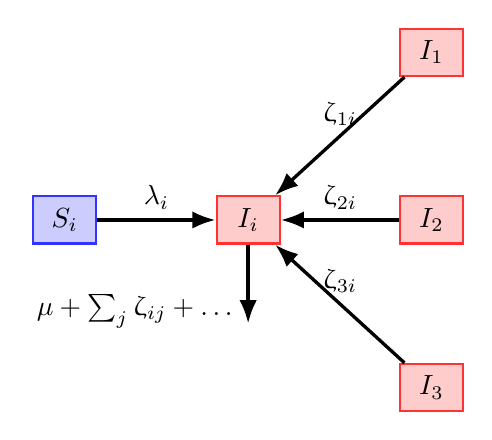
\begin{tikzpicture}
  \node(y)[tbox=red] {$I_i$};
  \node(s)[tbox=blue, left = of y]{$S_i$};
  \node(b)[tbox=red, right = of y]{$I_2$};
  \node(a)[tbox=red, above = of b]{$I_1$};
  \node(c)[tbox=red, below = of b]{$I_3$};
  \node(x)[below = of y]{};
  \draw[arrow,<-] (y) -- node[above] {$\lambda_{i}$} (s);
  \draw[arrow,<-] (y) -- node[above] {$\zeta_{1i}$} (a);
  \draw[arrow,<-] (y) -- node[above] {$\zeta_{2i}$} (b);
  \draw[arrow,<-] (y) -- node[above] {$\zeta_{3i}$} (c);
  \draw[arrow,->] (y) -- node[below left] {$\mu + \sum_j{\zeta_{ij}} + \dots$} (x);
\end{tikzpicture}
  \caption{System of compartments and flows between them for $\G = 3$}
  \label{fig:system}
\end{figure}
\par
Some key assumptions of this work:
\begin{itemize}
  \item The health states of individuals moving between risk groups due to turnover
  is proportional to the health states of the group overall.
  \item Disease-attributable death has negligible impact on risk-group proportions.
  \item 
\end{itemize}
% ==================================================================================================
\subsection{Parameterization}\label{ss:params}
Next, we explore methods for estimating the values of parameters
in the system described above
($\nu$, $\mu$, $\bm{\hat{x}}$, $\bm{\hat{e}}$, and $\zeta$)
directly from some commonly available sources of data.
\par
In most cases, there will not be sufficient data to directly estimate all parameters,
especially $\zeta$.
The next section outlines additional methods to solve for these values.
% * (is this true anymore?)
% * (discuss latent assumptions with each of these approaches)
% --------------------------------------------------------------------------------------------------
\subsubsection{Total Population Size}\label{sss:params-nu-mu}
%\begin{table}
%  \centering
%  \caption{Methods for deriving entry $\nu$ and exit $\mu$ rates}
%  \label{tab:nu-mu}
%  \begin{tabular}{lclll}
	\toprule
	Parameter       &    Symbol    & Data Sources & Key Equations & Validation \\
	\midrule
	Population Size &   $\N(t)$    &              &               &            \\
	Growth rate     & $\growth(t)$ &              &               &            \\
	Entry rate      &   $\nu(t)$   &              &               &            \\
	Exit rate       &   $\mu(t)$   &              &               &            \\
	\bottomrule
\end{tabular}
%\end{table}
The model of total population size over time is defined by
entry and exit rates, $\nu$ and $\mu$, as in:
\begin{subequations}
  \begin{align}
  \N(t) &= \N_0 {\big(1+\mathcal{G}(t)\big)}^{t} \label{eq:growth-N}\\
  \mathcal{G}(t) &= \nu(t) - \mu(t)              \label{eq:growth-G}
  \end{align}
\end{subequations}
and we note that the average duration of an individual in the model at time $t$
is given by:
\begin{equation} \label{eq:duration-model}
  \delta(t) = \mu^{-1}(t)
\end{equation}
Variation in rate of entry across risk groups is captured in $\bm{\hat{e}}$,
and we generally do not stratify rate of exit by activity group
(besides disease-attributable death);
therefore, we can assume that $\nu$ and $\mu$ do not vary across risk groups,
which allows us to derive them with $\N(t)$, independent of
the population proportions $\bm{\hat{x}}$, $\bm{\hat{e}}$, and turnover $\zeta$.
\par
The simplest approach assumes a constant population size $\N(t) = \N_0$,
or a growth rate of zero, yielding $\nu = \mu$.
However, this does not reflect the true positive population growth of most contexts,
and may result in underestimated incidence,
due to the relative reduction in inflow of susceptibles.
% verified in code, see:
% https://github.com/c-uhs/turnover/blob/f029bd1/outputs/figs/debug/incidence-nu.gif
\par
Another approach is to fix $\mathcal{G}(t)$ as some constant.
When using this approach, extra care should be taken to ensure
the resulting $\N(t)$ matches any available population size estimates to a reasonable degree.
\par
Typically, data will be available for the total size of the population over time $\N(t)$,
so the growth rate for each time interval $t_i$
can be derived by rearranging \eq{eq:growth-N}:
\begin{equation}
\mathcal{G}(t_i) = {\left(\frac{\N(t_{i+1})}{\N(t_{i})}\right)}^{-(t_{i+1}-t_i)} - 1
\end{equation}
All of these approaches help define $\mathcal{G}(t)$, but leave one degree of freedom,
since any choice of $\mu(t)$ can be compensated by $\nu(t)$ to yield the desired $\mathcal{G}(t)$.
However, we can usually leverage the known duration of individuals in the model $\delta(t)$
to choose $\mu(t)$ as in \eq{eq:duration-model}.
This can come from an assumed duration of sexual activity,
or a constant, predefined age range relevant to parameterization.
Then, we can solve for $\nu(t)$ using \eq{eq:growth-G}.
% --------------------------------------------------------------------------------------------------
\subsubsection{Turnover}\label{sss:params-turnover}
% TODO: discuss common approaches - especially turnover is constant, or zero.
% TODO: discuss more the assumptions throughout.
Next, we assume that $\nu(t)$ and $\mu(t)$ are known,
and we focus on resolving $\bm{\hat{e}}(t)$ and $\zeta(t)$.
Similar to above, we will first formulate the problem as a system of equations;
then we will consider which data and assumptions we can leverage to solve the system.
\par
We begin by defining the ``conservation of mass'' equation for a given group $x_i$,
where that the rate of change of the group
is simply the sum of flows in~/~out of the group:
\begin{equation}\label{eq:mass-balance}
\frac{d}{dt}x_i
= \nu \thinspace e_i + \sum_{j}{\zeta_{ji} \thinspace x_j}
- \mu \thinspace x_i - \sum_{j}{\zeta_{ij} \thinspace x_i}
\end{equation}
While \eq{eq:mass-balance} is written in terms of
absolute population sizes $\bm{x}$ and $\bm{e}$,
it is equivalent to divide through by $\N$, yielding a system in terms of
proportions $\bm{\hat{x}}$ and $\bm{\hat{e}}$,
which is often more useful, since $\N$ need not be known.
\par
We further assume that the average proportions of each group $\hat{x}_i$ do not change over time.
Therefore, the desired rate of change for risk group $i$
will be equal to the growth of the risk group, $\mathcal{G} x_i$.
Substituting this into \eq{eq:mass-balance},
and simplifying, we have:
%we have:
%\begin{equation}
%\mathcal{G} x_i = \nu \thinspace e_i + \sum_{j}{\zeta_{ji} \thinspace x_j}
%- \mu \thinspace x_i - \sum_{j}{\zeta_{ij} \thinspace x_i}
%\end{equation}
%which, using the definition of $\mathcal{G}$ in \eq{eq:growth-G}, we can simplify to:
\begin{equation}\label{eq:system}
\nu \thinspace x_i
= \nu \thinspace e_i + \sum_{j}{\zeta_{ji} \thinspace x_j}
- \sum_{j}{\zeta_{ij} \thinspace x_i}
\end{equation}
Now, depending on the number of risk groups, we have
$\G$ and $\G(\G-1)$ unknowns in $\bm{e}$ and $\zeta$, totalling $\G^2$ variables to resolve.
We denote these variables as the vector $\bm{\theta} = \left[\bm{e}, \bm{z}\right]$,
where $\bm{z} = \mathrm{vec}_{i \ne j}(\zeta)$;
this allows us to define
a system of linear equations of the form:
\begin{equation}
\bm{b} = A \thinspace \bm{\theta}
\end{equation}
where $A$ is a $\G \times \G^2 $ matrix
and $\bm{b}$ is a $\G$-length vector,
representing the right-hand side and left-hand side of \eq{eq:system}, respectively.
In this form, we can use $A^{-1}\bm{b} = \bm{\theta}$ to solve for $\bm{\theta}$.
\par
Unfortunately, for any $\G > 1$, the system is underdetermined by a factor of $\G(\G-1)$,
meaning there are many combinations of $\bm{e}$ and $\zeta$ which satisfy \eq{eq:system}.
Therefore, we now resume our task of leveraging data and assumptions
to define a unique solution.
\par
Our first tool is another equation.
We note that the duration of time spent in a particular group $\delta_i$
is the inverse of all efferent flow rates:
\begin{equation}\label{eq:duration-group}
\delta_i = {\bigg(\mu + \sum_{j}{\zeta_{ij}}\bigg)}^{-1}
\end{equation}
These durations could be derived from survey data, including for key populations,
or they could be assumed.
Rearranging \eq{eq:duration-group}, we obtain
${\delta_i}^{-1} - \mu = \sum_{j}{\zeta_{ij}}$,
which yields an additional $\G$ equations in our linear system -- i.e.\ rows of $A$ and $\bm{b}$.
For $\G = 2$, this provides enough constraints to fully determine the system,
as shown in \app{a:example-systems},
but for larger $\G$, still more constraints are needed.
\par
The simplest additional constraints can be elements in $\bm{\theta}$ which are directly specified
-- i.e.\ elements of of $\bm{e}$ or $\zeta$.
For example, the proportion of individuals who
move from one risk group to another each year ($\zeta_{ij}$)
may be assumed or derived from data.
Similarly, the distribution of individuals
across risk groups in the entering population $\bm{\hat{e}}$
may be approximated using the proportions among
the lowest age group for which data are available.
In each case, the value specified is appended to $\bm{b}$,
and a row appended to $A$ of the form: $[0,\dots,1,\dots,0]$,
with $1$ in the position of the element in $\bm{\theta}$.
\par
There are, however, two notable caveats to this approach.
First, not all combinations of specified elements will add an equal number of constraints.
Specifying all elements of $\bm{e}$
will only add $\G-1$ (not $\G$) constraints,
since $\sum \bm{\hat{e}} = 1$, so the final element adds no new information.
Similarly, specifying all elements of $\zeta_{ij}$ for a given $i$
as well as the duration for the group $\delta_i$
will only add $\G-1$ (not $\G$) constraints,
since \eq{eq:duration-group} must hold.
%\footnote{Recall that the diagonal elements of $\zeta$ are inconsequential,
%  so only $\G-1$ elements of $\zeta_{ij}$ may be specified at all for a given $i$.}
Second, not all combinations of specified values will yield a valid solution,%
\footnote{Even rank-deficient systems be inconsistent.}
and it is unfortunately difficult to anticipate problematic combinations.
\par
Finally, we note that additional constraints may be avoided altogether if we pose the problem
as an optimization problem, namely:
\begin{equation}\label{eq:system-optimize}
\bm{\theta}^{*} = {\arg \min}
  \thinspace f(\bm{\theta}),
  \quad \textrm{subject to:}
  \enspace\bm{b} = A\thinspace\bm{\theta};
  \enspace\bm{\theta} \ge 0
\end{equation}
where $f$ is a function such as ${\left|\left| \thinspace\cdot\thinspace \right|\right|}_2$.
However, the choice of $f$ implies a prior on the values of $\bm{\theta}$,
and so introduces bias in the solution.
% ==================================================================================================
\subsection{Previous Approaches}
In this section, we will examine previous approaches to modelling
risk groups in simulated HIV epidemics,
and the assumptions inherent to these methods.
Box~\ref{box:assumptions} summarizes
the most common assumptions regarding the dynamics of these risk groups,
while Table~\ref{tab:prior-work} summarizes previous works
with respect to these assumptions.
\par
Many of the previously proposed models of HIV transmission
follow Assumption~\ref{ass:risk-groups-no} and do not consider heterogeneity
in risk of acquisition within major demographic groups,
such as heterosexual men / women, and MSM.
This is a significant assumption,
and may lead to large discrepancies with models which do consider risk heterogeneity,
as explored in Section~\ref{s:exp}.
Moreover, this assumption precludes any consideration of turnover,
since there is only one risk group, $\G = 1$.
\par
* (discussion of each assumption in turn)
\begin{floatbox}
  \caption{Common assumptions regarding the dynamics of risk groups}
  \label{box:assumptions}
  \begin{fboxed}
  \begin{enumerate}[leftmargin=1em]
    \item\label{ass:risk-groups}\textbf{Risk Groups:}
    Populations are stratified by risk of infection acquisition.
    \begin{enumerate}
      \item\label{ass:risk-groups-no}\textbf{No:} $G = 1$;
      Populations are homogeneous in risk of infection acquisition.
      \item\label{ass:risk-groups-yes}\textbf{Yes:} $G > 1$;
      Heterogeneity in risk of infection acquisition within populations is considered.
    \end{enumerate}
    \item\label{ass:turnover}\textbf{Turnover:}
    Individuals may move between risk groups.
    \begin{enumerate}
      \item\textbf{No:} $\zeta = 0$;
      Individuals do not move between risk groups.
      \item\textbf{Constant:} $\zeta > 0$;
      Individuals move between risk groups at a constant rate.
%      \item\textbf{Dynamic:} $\zeta = f$;
%      Individuals move between risk groups in dynamically.
    \end{enumerate}
    \item\label{ass:pop-growth}\textbf{Population Growth:}
    Increase in the total $N$ over time.
    \begin{enumerate}
      \item\textbf{No:} $\nu = \mu$;
      Population size $N$ is constant.
      \item\textbf{Yes:} $\nu > \mu$;
      Population size $N$ increases, at some constant or data-driven rate.
    \end{enumerate}
  \end{enumerate}
\end{fboxed}

\end{floatbox}
\begin{table}
  \centering
  \caption{Summary of prior work with respect to modelled risk group dynamics.}
  \label{tab:prior-work}
  \input{tabs/tab-prior-work.tex}
\end{table}
\clearpage
%%%%%%%%%%%%%%%%%%%%%%%%%%%%%%%%%%%%%%%%%%%%%%%%%%%%%%%%%%%%%%%%%%%%%%%%%%%%%%%%%%%%%%%%%%%%%%%%%%%%
\section{Experiment}\label{s:exp}
We have described an approach to parameterizing models of risk group dynamics
which hopefully highlights the
\textit{feasibility} of including such model components based on available data.
Next, we will explore the
\textit{importance} of including these components
through comparison of projected model outputs
across different implementations of risk group dynamics.
First, we will compare major structural variants
involving population growth, risk groups, and turnover.
Second, we will investigate the impact of turnover sparsity
-- that is, only modelling certain transitions,
such as in~\cite{Eaton2014}.
% ==================================================================================================
\subsection{Model \& Simulations}\label{ss:model}
We use a simple deterministic model of heterosexual HIV transmission,
including three health states:
susceptible~$\mathcal{S}$, infected~$\mathcal{I}$, and on treatment~$\mathcal{T}$,
as shown in Figure~\ref{fig:health-states},
and up to three levels of sexual activity (risk groups $\G$):
high~$H$, medium~$M$, and low~$L$.
Individuals of sex $\mathit{k}$ in risk group $i$ are assumed to
form sexual partnerships at a rate $C_{ki}$
with individuals of the opposite sex $\mathrm{k}$.
The probability of partnership formation with
a partner of sex $\mathrm{k}$ in risk group $\mathrm{i}$
is assumed to follow
the formulation proposed by \citeauthor{Garnett1994}~\cite{Garnett1994}:
\begin{equation}
  \rho_{\mathit{ki}\mathrm{ki}} =
  (1-\epsilon)\psi_{\mathit{ki}\mathrm{ki}}
   +(\epsilon)\pi_{\mathit{ki}\mathrm{ki}}
\end{equation}
where $\epsilon$ is a parameter controlling the dominance of
assortative $\psi$ ($\epsilon = 0$) versus proportional $\pi$ ($\epsilon = 1$) mixing.
\begin{figure}
  \centering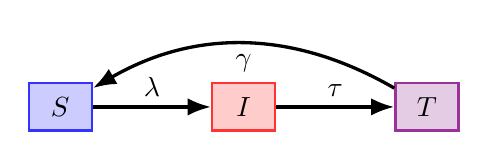
\begin{tikzpicture}
\node(S) [tbox=blue] at (0.0,0.0)   {$S$};
\node(I) [tbox=red,    right = of S]{$I$};
\node(T) [tbox=violet, right = of I]{$T$};

\draw[arrow=black] (S) edge["$\lambda$"] (I);
\draw[arrow=black] (I) edge["$\tau$"]  (T);
\draw[arrow=black] (T) edge["$\gamma$", bend right] (S);
\end{tikzpicture}
  \caption{Modelled health states}\label{fig:health-states}
\end{figure}
\par
Transmission of HIV from infected $\mathcal{I}$ to susceptible $\mathcal{S}$ individuals
is assumed to occur with probability $\beta_{\mathit{k}\mathrm{k}}$ per partnership.
Individuals on treatment $\mathcal{T}$ are not considered infectious.
The force of infection for susceptibles of sex $k$ in risk group $i$
is therefore modelled using the following equation:%~\cite{?}
\begin{equation}
  \lambda_{ki} =
  C_{\mathit{ki}}
  \sum_{\mathrm{ki}}
  \rho_{\mathit{ki}\mathrm{ki}} \thinspace
  \beta_{\mathit{k}\mathrm{k}}
  \frac{\mathcal{I}_{\mathrm{ki}}}{\N_{\mathrm{ki}}}
\end{equation}
Infected individuals are assumed to be diagnosed and begin treatment at a rate $\tau$ (per year).
As described in Section \ref{s:system},
individuals enter the model at a rate $\nu$,
exit at a rate $\mu$,
and transition between risk groups at rates $\zeta_{ij}$.
The default parameters for this base model are summarized in
Table~\ref{tab:params-base}.
\begin{table}[b]
  \centering\caption{Base model parameters. All rates have units $\mathrm{year}^{-1}$ and durations are in $\mathrm{years}$.}
  \label{tab:params-base}
  \begin{tabular}{clc}
	\toprule
	    Symbol     & Description                                                                                             &         Value         \\
	\midrule
	   $\beta$     & transmission probability per partnership: men $\rightarrow$ women, women $\rightarrow$ men              &    \tarr{0.1,0.05}    \\
	  $\epsilon$   & mixing parameter where: 1 $\rightarrow$ proportional and 0 $\rightarrow$ assortative \cite{Garnett1994} &          1.0          \\
	    $\tau$     & rate of treatment initiation among infected                                                             &          0.1          \\
	    $\N_0$     & initial population size                                                                                 &         1000          \\
	\midrule
	$\bm{\hat{x}}$ & proportion of system individuals: high, medium, low activity                                            & \tarr{0.04,0.20,0.76} \\
	$\bm{\hat{e}}$ & proportion of entering individuals: high, medium, low activity                                          & \tarr{0.04,0.20,0.76} \\
	$\bm{\delta}$  & average duration spent in: high, medium, and low activity groups                                        &    \tarr{5,15,25}     \\
	     $C$       & rate of partner change among individuals: high, medium, low activity                                    &     \tarr{25,5,1}     \\
	    $\nu$      & rate of population entry                                                                                &         0.05          \\
	    $\mu$      & rate of population exit                                                                                 &         0.03          \\
	\bottomrule
\end{tabular}
\end{table}
\par
Using this model (and its variants),
simulated epidemics are initialized in $t = 1975$ with $\N_0 = 1000$ individuals,
distributed proportionally according to $\bm{\hat{x}}$.
Among these individuals, 6 are infected, and the remainder are susceptible;
for $\G = 3$, this corresponds to one infected person in each sex-risk group,
while for $\G = 1$, this corresponds to three infected people in each sex.
Simulated epidemics run until $t = 2025$,
and are solved numerically using Euler's method with a time step of $dt = 0.5$ years.
% ==================================================================================================
\subsection{Structural Variants}\label{ss:structure-variants}
Drawing on the most common assumptions outlined in Box~\ref{box:assumptions},
we define a series of six structural model variants (S1~--~S6) for investigation.
These variants, summarized in Figure~\ref{fig:variant-tree}, include
zero versus nonzero population growth,
homogeneous versus heterogeneous risk ($\G = 1$ vs $\G = 3$),
and zero versus nonzero turnover among risk groups ($\zeta = 0$ vs $\zeta > 0$).
\begin{figure}
  \centering\newlength{\lvl}\setlength{\lvl}{1.2cm}
%\begin{tikzpicture}[
%    level distance = \lvl,
%    edge from parent/.append style = { draw = none } 
%  ]
%  \Tree [.{} [.{$\G$} [.{$\zeta$} ] ] ] 
%\end{tikzpicture}\hspace{0.5\lvl}
\begin{tikzpicture}[
    level distance = \lvl,
    sibling distance = 0.4\lvl,
    every path/.append style = { thick },
    edge from parent path = {
      (\tikzparentnode) -- +(0.0,-0.5\lvl) -| (\tikzchildnode)
    }
  ]
  \Tree
    [.{}
      [.\node[leaf=gray]{$\G=1$};
        [.\node[leaf=gray]{$\cdot$}; ]
      ]
      [.\node[leaf=gray]{$\G=3$};
        [.\node[leaf=gray]{$\zeta = 0$}; ]
        [.\node[leaf=gray]{$\zeta = C$}; ]
      ]
    ]
\end{tikzpicture}

  \caption{Summary of 6 structural model variants with respect to simulated risk group dynamics.
    $\nu$:~rate of population entry,
    $\mu$:~rate of population exit,
    $\G$:~number of risk groups,
    $\zeta$:~rates of population turnover}
  \label{fig:variant-tree}
\end{figure}
\par
In order to facilitate fair comparisons across model variants with respect to parameter values,
we start from the base model described above (S1~in Figure~\ref{fig:variant-tree}),
and aim to make simplifications with minimal impact on system characteristics.
% not sure how to communicate this idea...
For example, when moving from $\nu > \mu$ to $\nu = \mu$,
we ensure the average duration of individuals in the model $\mu^{-1}$ is unchanged
by fixing $\mu$ and reducing $\nu$ to match (S4~--~S6).
Similarly, when collapsing the stratification of risk groups from $\G = 3$ to $\G = 1$ (S3,~S6),
we define the homogeneous partner change rate $C$
as the weighted average of the previously risk-stratified $C$.
Finally, considering rates of turnover $\zeta$
(which are only applicable for S1,~S4)
we fully determine the system, as outlined in Section~\ref{sss:params-turnover},
by specifying the average duration of individuals in each group $\bm{\delta}$,
as well as the distribution of individuals entering the model $\bm{\hat{e}}$,
and the proportion of high activity individuals moving to the low activity group each year $\zeta_{HL}$.
The resulting parameter values for each scenario
are summarized in Table~\ref{tab:params-structure}.
\begin{table}
  \centering\caption{Model parameters for structural variants.
    All rates have units $\mathrm{year}^{-1}$ and durations are in $\mathrm{years}$.}
  \label{tab:params-structure}
  \begin{tabular}{ccccccc}
	\toprule
	  Parameter    &          S1           &          S2           &     S3      &          S4           &          S5           &     S6      \\
	\midrule
	$\bm{\hat{x}}$ & \tarr{0.04,0.20,0.76} & \tarr{0.04,0.20,0.76} & \tarr{1.0}  & \tarr{0.04,0.20,0.76} & \tarr{0.04,0.20,0.76} & \tarr{1.0}  \\
	$\bm{\hat{e}}$ & \tarr{0.04,0.20,0.76} & \tarr{0.04,0.20,0.76} & \tarr{1.0}  & \tarr{0.04,0.20,0.76} & \tarr{0.04,0.20,0.76} & \tarr{1.0}  \\
	     $C$       &     \tarr{25,5,1}     &     \tarr{25,5,1}     & \tarr{2.76} &     \tarr{25,5,1}     &     \tarr{25,5,1}     & \tarr{2.76} \\
	   $\delta$    &    \tarr{5,15,25}     &    \tarr{33,33,33}    &  \tarr{33}  &    \tarr{5,15,25}     &    \tarr{33,33,33}    &  \tarr{33}  \\
	 $\zeta_{HL}$  &         0.10          &         0.10          &    0.10     &         0.10          &         0.10          &    0.10     \\
	    $\nu$      &         0.05          &         0.05          &    0.05     &         0.03          &         0.03          &    0.03     \\
	    $\mu$      &         0.03          &         0.03          &    0.03     &         0.03          &         0.03          &    0.03     \\
	\bottomrule
\end{tabular}
\end{table}
% ==================================================================================================
\subsection{Turnover Variants}\label{ss:zeta-variants}
While implementing the complete system described in Section~\ref{s:system}
affords potential improvements in model accuracy,
parameterizing such a system poses several challenges,
such as data availability
and combining constraints to yield a fully determined system.
As such, it may be tempting to implement only some turnover transitions.
In the current framework, this equates to setting some elements in $\zeta$ to zero.
However, such an approach may introduce bias in the results.
This section introduces seven model variants (Z0~--~Z6) with respect to sparsity of $\zeta$,
to explore this possibility.
\par
Variant Z0 has no turnover, making it identical to S2,
while variant Z6 includes all transitions, making it very similar to S1
(transition rates are slightly different).
Variants Z1 through Z5 then represent models ``in between'' S1 and S2,
with Z1~--~Z3 adding flows from higher activity groups to lower activity groups,
and Z4~--~Z6 adding the reverse flows.
A summary of the corresponding turnover matrices $\zeta$,
as well as the necessary constraints to obtain a unique solution ($\bm{\hat{e}}$, $\bm{\delta}$),
are given in Table~\ref{tab:params-zeta}.
\begin{table} % TODO: change notation of "z_i" in this table, as it conflicts with z = vec(\zeta)
  \centering\caption{Model parameters for turnover variants.
    All rates have units $\mathrm{year}^{-1}$ and durations are in $\mathrm{years}$.}
  \label{tab:params-zeta}
  {
\newcommand{\mzeta}[6]{%
  \def\arraycolsep{3pt}
  $\left[\begin{matrix}
  \cdot & #1    & #2    \\
  #3    & \cdot & #4    \\
  #5    & #6    & \cdot \\
  \end{matrix}\right]$}
\begin{tabular}{cccccccc}\toprule
  Parameter & Z0 & Z1 & Z2 & Z3 & Z4 & Z5 & Z6 \\\midrule
  $\zeta$: & 
  \mzeta{ 0 }{ 0 }{ 0 }{ 0 }{ 0 }{ 0 } &
  \mzeta{ 0 }{ * }{ 0 }{ 0 }{ 0 }{ 0 } &
  \mzeta{z_1}{z_1}{ 0 }{ 0 }{ 0 }{ 0 } & 
  \mzeta{z_1}{z_1}{ 0 }{ * }{ 0 }{ 0 } &
  \mzeta{z_1}{z_1}{ 0 }{ * }{ * }{ 0 } &
  \mzeta{z_1}{z_1}{ 0 }{ * }{z_3}{z_3} &
  \mzeta{z_1}{z_1}{z_2}{z_2}{z_3}{z_3} 
  \\[2em]
  $\bm{\hat{e}}$: & 
  \tarr{*,*,*} &
  \tarr{*,*,*} &
  \tarr{*,*,*} &
  \tarr{*,*,*} &
  \tarr{*,*,*} &
  \tarr{*,*,*} &
  \tarr{*,*,*}
  \\[1em]
  $\bm{\delta}$: &
  \tarr{    *   ,    *   ,    *   } &
  \tarr{\delta_1,    *   ,    *   } &
  \tarr{\delta_1,    *   ,    *   } &
  \tarr{\delta_1,\delta_2,    *   } &
  \tarr{\delta_1,\delta_2,\delta_3} &
  \tarr{\delta_1,\delta_2,\delta_3} &
  \tarr{\delta_1,\delta_2,\delta_3}
  \\\bottomrule
\end{tabular}\\[0.5em]
$z_i$, $e_i$, $\delta_i$: specified values;
$(*)$: calculated values;
$(\cdot)\thinspace$: inconsequential.\\
$z_1 = 0.085$, $z_2 = 0.0183$, $z_3 = 0.005$;
$\delta_1 = 5$, $\delta_2 = 15$, $\delta_3 = 25$.
}
\end{table}
% ==================================================================================================
%\subsection{Simulations}
%For each of the model structures described above,
%we simulate ...
%
%\par
%%This epidemic was simulated
%%using each of the model variants described in \S~\ref{ss:model-variants}.
%%In each case, we compared the model predictions across the variants
%%regarding three outputs:
%\begin{enumerate}
%  \item Projected prevalence for $t = 1975 - 2050$
%  \item Population attributable fraction of highest risk group (variants with $\G = 3$ only)
%  \item Estimated impact of \{intervention x -- ART?\}
%  at reducing cumulative new infections between 2020 and 2050
%\end{enumerate}
%\dots
%\par
%Since the results of these comparisons are significantly affected by several model parameters,
%we performed a comprehensive sensitivity analysis.
%The parameter ranges specified in Table~\ref{tab:base-model-params} were used,
%and \dots
%* (construct a GLM or something to describe the impacts?)
%%%%%%%%%%%%%%%%%%%%%%%%%%%%%%%%%%%%%%%%%%%%%%%%%%%%%%%%%%%%%%%%%%%%%%%%%%%%%%%%%%%%%%%%%%%%%%%%%%%%
%\section{Results}\label{s:results}
%\begin{figure}
%  \centering\scalebox{6}{$\times$}
%%  \centering\includegraphics[width=0.4\textwidth]{{cum-infect_nu=0.03_G=1_Z=0}.pdf}
%  \caption{Projected prevalence under each of the 10 model variants.}
%\end{figure}
%\begin{figure}
%  \centering\scalebox{6}{$\times$}
%  \caption{Estimated impact of \{intervention x\} on
%    cumulative new infections between 2020 and 2050.}
%\end{figure}
%%%%%%%%%%%%%%%%%%%%%%%%%%%%%%%%%%%%%%%%%%%%%%%%%%%%%%%%%%%%%%%%%%%%%%%%%%%%%%%%%%%%%%%%%%%%%%%%%%%%
%\section{Discussion}\label{s:discussion}
% ideas
% - limitations
%   - have not considered differential death -> dynamic recalculation possible solution
%     - but which assumption is more plausible: (1) constant x -> adaptive zeta?
%                                               (2) constant zeta -> changes in x with attr death?
%   - 
%%%%%%%%%%%%%%%%%%%%%%%%%%%%%%%%%%%%%%%%%%%%%%%%%%%%%%%%%%%%%%%%%%%%%%%%%%%%%%%%%%%%%%%%%%%%%%%%%%%%
%\section{Conclusions}\label{s:conclusion}
\clearpage
%%%%%%%%%%%%%%%%%%%%%%%%%%%%%%%%%%%%%%%%%%%%%%%%%%%%%%%%%%%%%%%%%%%%%%%%%%%%%%%%%%%%%%%%%%%%%%%%%%%%
\section{References}\label{s:references}
\printbibliography[heading=none]
%%%%%%%%%%%%%%%%%%%%%%%%%%%%%%%%%%%%%%%%%%%%%%%%%%%%%%%%%%%%%%%%%%%%%%%%%%%%%%%%%%%%%%%%%%%%%%%%%%%%
\clearpage\appendix
%%%%%%%%%%%%%%%%%%%%%%%%%%%%%%%%%%%%%%%%%%%%%%%%%%%%%%%%%%%%%%%%%%%%%%%%%%%%%%%%%%%%%%%%%%%%%%%%%%%%
\section{Example Systems}\label{a:example-systems}
% ==================================================================================================
\subsection{$\G = 1$}
\begin{equation}
\left[\begin{array}{c}
	\nu x_1
\end{array}\right]
=
\left[\begin{array}{c}
	\nu
\end{array}\right]
\left[\begin{array}{c}
	e_1
\end{array}\right]
\end{equation}
% ==================================================================================================
\subsection{$\G = 2$}
\begin{equation}
\left[\begin{array}{c}
	       \nu x_1        \\
	       \nu x_2        \\
	{\delta_1}^{-1} - \mu \\
	{\delta_2}^{-1} - \mu
\end{array}\right]
=
\left[\begin{array}{cccc}
	 \nu  & \cdot & -x_1  &  x_2  \\
	\cdot &  \nu  &  x_1  & -x_2  \\
	\cdot & \cdot &   1   & \cdot \\
	\cdot & \cdot & \cdot &   1
\end{array}\right]
\left[\begin{array}{c}
	   e_1     \\
	   e_2     \\
	\zeta_{12} \\
	\zeta_{21}
\end{array}\right]
\end{equation}
% ==================================================================================================
\subsection{$\G = 3$}
\begin{equation}
\left[\begin{array}{c}
	       \nu x_1        \\
	       \nu x_2        \\
	       \nu x_3        \\
	{\delta_1}^{-1} - \mu \\
	{\delta_2}^{-1} - \mu \\
	{\delta_3}^{-1} - \mu \\
%	        e^*_1         \\
%	        e^*_2         \\
%	        e^*_3         \\
\end{array}\right]
=
\left[\begin{array}{ccccccccc}
	 \nu  & \cdot & \cdot & -x_1  & -x_1  &  x_2  & \cdot &  x_3  & \cdot \\
	\cdot &  \nu  & \cdot &  x_1  & \cdot & -x_2  & -x_2  & \cdot &  x_3  \\
	\cdot & \cdot &  \nu  & \cdot &  x_1  & \cdot &  x_2  & -x_3  & -x_3  \\
	\cdot & \cdot & \cdot &   1   &   1   & \cdot & \cdot & \cdot & \cdot \\
	\cdot & \cdot & \cdot & \cdot & \cdot &   1   &   1   & \cdot & \cdot \\
	\cdot & \cdot & \cdot & \cdot & \cdot & \cdot & \cdot &   1   &   1   \\
%	  1   & \cdot & \cdot & \cdot & \cdot & \cdot & \cdot & \cdot & \cdot \\
%	\cdot &   1   & \cdot & \cdot & \cdot & \cdot & \cdot & \cdot & \cdot \\
%	\cdot & \cdot &   1   & \cdot & \cdot & \cdot & \cdot & \cdot & \cdot \\
\end{array}\right]
\left[\begin{array}{c}
	   e_1     \\
	   e_2     \\
	   e_3     \\
	\zeta_{12} \\
	\zeta_{13} \\
	\zeta_{21} \\
	\zeta_{23} \\
	\zeta_{31} \\
	\zeta_{32} \\
\end{array}\right]
\end{equation}
%% ==================================================================================================
%\subsection{$\G = 4$}
%\begin{equation}
\left[\begin{array}{c}
	         \nu x_1           \\
	         \nu x_2           \\
	         \nu x_3           \\
	         \nu x_4           \\
	{\mathcal{D}_1}^{-1} - \mu \\
	{\mathcal{D}_2}^{-1} - \mu \\
	{\mathcal{D}_3}^{-1} - \mu \\
  {\mathcal{D}_4}^{-1} - \mu
\end{array}\right]
=
\left[\begin{array}{cccccccccccccccc}
	 \nu  & \cdot & \cdot & \cdot & -x_1  & -x_1  & -x_1  &  x_2  & \cdot & \cdot &  x_3  & \cdot & \cdot &  x_4  &       &       \\
	\cdot &  \nu  & \cdot & \cdot &  x_1  & \cdot & \cdot & -x_2  & -x_2  & -x_2  & \cdot &  x_3  & \cdot &       &  x_4  &       \\
	\cdot & \cdot &  \nu  & \cdot & \cdot &  x_1  & \cdot & \cdot &  x_2  & \cdot & -x_3  & -x_3  & -x_3  &       &       &  x_4  \\
	\cdot & \cdot & \cdot &  \nu  & \cdot & \cdot &  x_1  & \cdot & \cdot &  x_2  & \cdot & \cdot &  x_3  & -x_4  & -x_4  & -x_4  \\
	\cdot & \cdot & \cdot & \cdot &   1   &   1   &   1   & \cdot & \cdot & \cdot & \cdot & \cdot & \cdot & \cdot & \cdot & \cdot \\
	\cdot & \cdot & \cdot & \cdot & \cdot & \cdot & \cdot &   1   &   1   &   1   & \cdot & \cdot & \cdot & \cdot & \cdot & \cdot \\
	\cdot & \cdot & \cdot & \cdot & \cdot & \cdot & \cdot & \cdot & \cdot & \cdot &   1   &   1   &   1   & \cdot & \cdot & \cdot \\
	\cdot & \cdot & \cdot & \cdot & \cdot & \cdot & \cdot & \cdot & \cdot & \cdot & \cdot & \cdot & \cdot &   1   &   1   &   1
\end{array}\right]
\left[\begin{array}{c}
	   e_1     \\
	   e_2     \\
	   e_3     \\
     e_4     \\
	\zeta_{12} \\
	\zeta_{13} \\
  \zeta_{14} \\
	\zeta_{21} \\
	\zeta_{23} \\
  \zeta_{23} \\
	\zeta_{31} \\
	\zeta_{32} \\
  \zeta_{34} \\
  \zeta_{41} \\
  \zeta_{42} \\
  \zeta_{43} \\
\end{array}\right]
\end{equation}
%%%%%%%%%%%%%%%%%%%%%%%%%%%%%%%%%%%%%%%%%%%%%%%%%%%%%%%%%%%%%%%%%%%%%%%%%%%%%%%%%%%%%%%%%%%%%%%%%%%%
\end{document}
%%%%%%%%%%%%%%%%%%%%%%%%%%%%%%%%%%%%%%%%%%%%%%%%%%%%%%%%%%%%%%%%%%%%%%%%%%%%%%%%%%%%%%%%%%%%%%%%%%%%
%%%%%%%%%%%%%%%%%%%%%%%%%%%%%%%%%%%%%%%%%%%%%%%%%%%%%%%%%%%%%%%%%%%%%%%%%%%%%%%%%%%%%%%%%%%%%%%%%%%%
%%%%%%%%%%%%%%%%%%%%%%%%%%%%%%%%%%%%%%%%%%%%%%%%%%%%%%%%%%%%%%%%%%%%%%%%%%%%%%%%%%%%%%%%%%%%%%%%%%%%